\id{IRSTI 81.93.29}

\begin{articleheader}
\sectionwithauthors{A.Zhumabekova, O.Ussatova, M.Kalimoldayev, V.Karyukin, Y Begimbayeva}{THE STUDY OF MACHINE AND DEEP LEARNING MODELS FOR MALWARE CLASSIFICATION}

{\bfseries \textsuperscript{1,2}A.Zhumabekova\textsuperscript{\envelope },
\textsuperscript{1,3}O.Ussatova, \textsuperscript{1}M.Kalimoldayev,
\textsuperscript{1,2}V.Karyukin,
\textsuperscript{1}}\textsuperscript{,{\bfseries 3}}{\bfseries Y Begimbayeva}
\end{articleheader}

\begin{affiliation}
\textsuperscript{1}Institute of Information and Computational
Technologies, Almaty, Kazakhstan,

\textsuperscript{2}Al-Farabi Kazakh National University, Almaty,
Kazakhstan,

\textsuperscript{3}G.Daukeev Almaty University of Energy and
Communications, Almaty, Kazakhstan

\raggedright {\bfseries \textsuperscript{\envelope }}Correspondent-author: \href{mailto:zhumabekova2702@gmail.com}{\nolinkurl{zhumabekova2702@gmail.com}}
\end{affiliation}

The rapid growth of cyber threats and attacks has highlighted the need
for robust information security, confidentiality, and integrity
measures. Malware, a significant category of cyber threats, is designed
to disrupt operations, damage information environments, and gain
unauthorized access to systems, networks, and data. Various types of
malware, including viruses, worms, trojans, spyware, and rootkits, pose
pervasive and evolving dangers, often spread through the Internet or
removable devices. While effective against known threats, traditional
signature-based detection methods struggle to identify new malware.
Modern machine learning-based approaches offer a more flexible solution
by learning from large datasets without relying on predefined
signatures. This research presents a machine learning-based malware
detection system using a dataset of diverse network threats. The study
explores both classical machine learning algorithms and advanced deep
learning models, including dense neural networks (DNN), Long Short-Term
Memory (LSTM) networks, and Gated Recurrent Units (GRU), to enhance
malware detection accuracy. Moreover, a newly developed hybrid LSTM-GRU
deep learning model was utilized for classifying the malware dataset.
This model combines the strong specifications of both LSTM and GRU
neural networks. The used machine learning and deep learning models
demonstrated good classification results. The Decision Tree, Random
Forest, and XGBoost machine learning models were superior to neural
networks by around 0.02. The experiments showed that machine learning
algorithms are still strong in the classification tasks of the
cybersecurity field. Among neural networks, the simple DNN model was a
little worse than LSTM and GRU by around 0.01. The recurrent LSTM and
GRU models showed mostly identical scores. The proposed LSTM-GRU model
outperformed other deep learning models by 0.01 and was comparable with
the Random Forest model that reached the metrics score of 0.99.

{\bfseries Keywords}: malware, information security, threat detection,
machine learning, deep learning, Chi-square, class balancing

\begin{articleheader}
{\bfseries ЗИЯНДЫ БАҒДАРЛАМАЛАРДЫ КЛАССИФИКАЦИЯЛАУ ҮШІН МАШИНАЛЫҚ ЖӘНЕ
ТЕРЕҢ ОҚУ МОДЕЛЬДЕРІН ЗЕРТТЕУ}

{\bfseries \textsuperscript{1,2}А.Жұмабекова\textsuperscript{\envelope },
\textsuperscript{1,3}О.Усатова, \textsuperscript{1}М.Қалимолдаев,
\textsuperscript{1,2}В.Карюкин, \textsuperscript{1,3}Е.Бегимбаева}
\end{articleheader}

\begin{affiliation}
\textsuperscript{1}Ақпараттық және есептеуіш технологиялар институты,
Алматы, Қазақстан,

\textsuperscript{2}әл-Фараби атындағы Қазақ Ұлттық Университеті, Алматы,
Қазақстан,

\textsuperscript{3}Ғ. Дәукеев атындағы Алматы энергетика және байланыс
университеті, Алматы, Қазақстан,

e-mail: zhumabekova2702@gmail.com
\end{affiliation}

Киберқауіптер мен шабуылдардың жылдам өсуі сенімді ақпараттық
қауіпсіздік, құпиялылық және тұтастық шараларының қажеттілігін көрсетті.
Зиянды бағдарламалар, киберқауіптердің маңызды санаты ақпараттық
орталарды бұзуға, зақымдауға және жүйелерге, желілерге және деректерге
рұқсатсыз кіруге арналған. Вирустар, құрттар, трояндар, шпиондық
бағдарламалар мен руткиттерді қоса алғанда, зиянды бағдарламалардың
әртүрлі түрлері Интернет немесе алынбалы құрылғылар арқылы жиі таралатын
кең таралған және дамып келе жатқан қауіп болып табылады. Қолтаңбаға
негізделген анықтаудың дәстүрлі әдістері белгілі қауіптерге қарсы тиімді
болғанымен, олар жаңа зиянды бағдарламаны анықтауда қиындықтарға тап
болады. Заманауи машиналық оқыту модельдері алдын ала анықталған
қолтаңбаларға сүйенбестен үлкен деректер жиынынан үйрену арқылы икемді
шешім ұсынады. Бұл зерттеу әртүрлі онлайн қауіптердің деректер жинағын
пайдалана отырып, машиналық оқытуға негізделген зиянды бағдарламаларды
анықтау жүйесін ұсынады. Жұмыс зиянды бағдарламаны анықтау дәлдігін
жақсарту үшін классикалық машиналық оқыту алгоритмдерін де, тереңдетіп
оқытудың кеңейтілген үлгілерін де, соның ішінде толық қосылған нейрондық
желілерді (DNN), ұзақ қысқа мерзімді жад желілерін (LSTM) және қақпалы
қайталанатын блоктарды (GRU) қарастырады. Сонымен қатар, зиянды
бағдарлама деректер жинағын жіктеу үшін жақында жасалған гибридті терең
оқыту үлгісі LSTM-GRU пайдаланылды. Бұл модель LSTM және GRU нейрондық
желілерінің күшті сипаттамаларын біріктіреді. Қолданылған машиналық
оқыту және терең оқыту үлгілері классификацияның жақсы нәтижелерін
көрсетті. Decision Tree, Random Forest және XGBoost машиналық оқыту
үлгілері нейрондық желілерден шамамен 0,02-ге асып түсті. Эксперименттер
машиналық оқыту алгоритмдері киберқауіпсіздік саласындағы жіктеу
тапсырмаларында әлі де күшті екенін көрсетті. Нейрондық желілер арасында
қарапайым DNN моделі LSTM және GRU-дан шамамен 0,01-ге нашар болды.
Қайталанатын LSTM және GRU үлгілері іс жүзінде бірдей бағалауларды
көрсетті. Ұсынылған LSTM-GRU моделі тереңдетіп оқытудың басқа
үлгілерінен 0,01-ге асып түсті және 0,99 метрикалық ұпайға қол жеткізген
Random Forest үлгісімен салыстыруға болатын. Эксперименттер машиналық
оқыту алгоритмдері киберқауіпсіздік саласындағы жіктеу тапсырмаларында
әлі де күшті екенін көрсетті. Нейрондық желілер арасында қарапайым DNN
моделі LSTM және GRU-дан шамамен 0,01-ге нашар болды. Қайталанатын LSTM
және GRU үлгілері іс жүзінде бірдей бағалауларды көрсетті. Ұсынылған
LSTM-GRU үлгісі басқа тереңдетіп оқыту үлгілерінен 0,01-ге асып түсті
және 0,99 метрикалық ұпайға қол жеткізген Random Forest үлгісімен
салыстыруға болатын.

{\bfseries Түйін сөздер:} Зиянды бағдарламалар, ақпараттық қауіпсіздік,
қауіпті анықтау, машиналық оқыту, терең оқыту, Chi-square, классты
теңдестіру

\begin{articleheader}
{\bfseries ИССЛЕДОВАНИЕ МОДЕЛЕЙ МАШИННОГО И ГЛУБОКОГО ОБУЧЕНИЯ ДЛЯ
КЛАССИФИКАЦИИ ВРЕДОНОСНОГО ПРОГРАММНОГО ОБЕСПЕЧЕНИЯ}

{\bfseries \textsuperscript{1,2}А.Жұмабекова\textsuperscript{\envelope },
\textsuperscript{1,3}О.Усатова, \textsuperscript{1}М.Қалимолдаев,
\textsuperscript{1,2}В.Карюкин, \textsuperscript{1,3}Е.Бегимбаева}
\end{articleheader}

\begin{affiliation}
¹Институт информационных и вычислительных технологий, Алматы, Казахстан,

²Казахский национальный университет имени аль-Фараби, Алматы, Казахстан,

³Алматинский университет энергетики и связи имени Г.Даукеева, Алматы, Казахстан,

e-mail: \href{mailto:zhumabekova2702@gmail.com}{\nolinkurl{zhumabekova2702@gmail.com}}
\end{affiliation}

Быстрый рост киберугроз и атак выявил необходимость в надежных мерах
информационной безопасности, конфиденциальности и целостности.
Вредоносное ПО, являясь значительной категорией киберугроз,
предназначено для нарушения работы, повреждения информационных сред и
получения несанкционированного доступа к системам, сетям и данным.
Различные виды вредоносного ПО, такие как вирусы, черви, трояны,
шпионские программы и руткиты, представляют собой все проникающие и
развивающиеся угрозы, часто распространяемые через интернет или съемные
устройства. Традиционные методы обнаружения, основанные на сигнатурах,
эффективны против известных угроз, но сталкиваются с трудностями в
идентификации нового вредоносного ПО. Современные методы машинного
обучения предлагают более гибкое решение, обучаясь на больших наборах
данных без необходимости использования заранее определенных сигнатур.
Данное исследование представляет систему обнаружения вредоносного ПО на
основе машинного обучения с использованием набора данных о различных
сетевых угрозах. В работе изучены как классические алгоритмы машинного
обучения, так и продвинутые модели глубокого обучения, включая
полносвязные нейронные сети (DNN), сети с длинной краткосрочной памятью
(LSTM) и рекуррентные блоки с управляемыми воротами (GRU), с целью
повышения точности обнаружения Вредоносного ПО. Более того, для
классификации датасета Вредоносного ПО использовалась недавно
разработанная гибридная модель глубокого обучения LSTM-GRU. Эта модель
сочетает в себе сильные характеристики нейронных сетей LSTM и GRU.
Используемые модели машинного обучения и глубокого обучения
продемонстрировали хорошие результаты классификации. Модели машинного
обучения Decision Tree, Random Forest и XGBoost превосходили нейронные
сети примерно на 0,02. Эксперименты показали, что алгоритмы машинного
обучения по-прежнему сильны в задачах классификации в области
кибербезопасности. Среди нейронных сетей простая модель DNN была немного
хуже LSTM и GRU примерно на 0,01. Рекуррентные модели LSTM и GRU
показали в основном идентичные оценки. Предложенная модель LSTM-GRU
превзошла другие модели глубокого обучения на 0,01 и была сопоставима с
моделью Random Forest, которая достигла оценки метрик 0,99. Эксперименты
показали, что алгоритмы машинного обучения по-прежнему сильны в задачах
классификации в области кибербезопасности. Среди нейронных сетей простая
модель DNN была немного хуже LSTM и GRU примерно на 0,01. Рекуррентные
модели LSTM и GRU показали в основном идентичные оценки. Предложенная
модель LSTM-GRU превзошла другие модели глубокого обучения на 0,01 и
была сопоставима с моделью Random Forest, которая достигла значений
метрик в 0,99.

{\bfseries Ключевые слова}: вредоносное ПО, информационная безопасность,
обнаружение угроз, машинное обучение, глубокое обучение, Chi-square,
балансировка классов.

\begin{multicols}{2}
{\bfseries Introduction.} Nowadays, the significant growth of different
types of cyber threats and attacks makes people seriously consider
possessing information security {[}1{]}, confidentiality {[}2{]}, and
integrity {[}3{]}. The specific characteristics of cyber threats belong
to malware. Malware is software designed to damage the information
environment, disrupt operations, and gain unauthorized system access,
network, and data. Malware {[}4{]} represents pervasive and dangerous
threats that evolve continuously to exploit vulnerabilities in
individual systems and large-scale networks. There is a great variety of
malware, including viruses (a type of malware that attaches itself to
legitimate files or programs), worms (self-replicating malware that can
spread across networks without needing to attach themselves to a host
file or program), trojans (this malware pretends to be legitimate
software and deceives users into downloading and executing them),
spyware (it monitors and collects information about users, such as
logins, passwords, credit card numbers, and other sensitive data),
rootkits (this malware is designed to give attackers the privilege to
access the system while hiding its presence), and different types of
threats.

Malware {[}5{]} is usually distributed via the Internet and removable
devices like flash drives. They affect systems by significantly reducing
the computer's performance, significantly reducing the free space of its
HDD and SSD drives, and displaying various advertisements on the screen.
This is one of the most obvious signs that the user's computer system is
infected with malware. Dangerous malware steals files containing
confidential data, hides them inside the computer, and continues to
perform malicious actions. In order to protect against malware, various
approaches are utilized. The signature-based approach is a traditional
method used by antivirus and anti-malware programs. It identifies unique
patterns, or signatures, associated with the known malware. During the
process of file scanning, the software compares its code to the
signature stored in the database. Although this approach can detect many
different types of malware, it also encounters problems with recognizing
new and previously unseen malware. A modern machine learning-based
method proposes a completely new way of detecting malware. It learns
from large datasets and does not rely on predefined signatures, which
makes it more flexible and capable of identifying previously unseen
malware.

The detection of malware with the use of machine and deep learning
approaches was explored in many scientific works. The paper {[}6{]}
focused on classifying malware with DNN and Bi-LSTM. The performance of
these two models was strong. DNN reached an accuracy score of 98\%,
while Bi-LSTM got 99\%. In the cybersecurity field, the work {[}7{]}
demonstrated a new machine-learning framework for detecting different
types of malware, including Ransomware, Spyware, and Trojan Horses. The
main algorithm of this framework was the Ensemble-based classifier that
proved effective in handling threats and reached an accuracy score of
98\%. The research paper {[}8{]} analyzes spyware detection using a
decision tree machine learning algorithm. It gave an opportunity to get
an accuracy score of 99\%. This classifier gave an accuracy score of
97\%, precision -- 88.9\%, recall -- 88.6\%, and F1-score -- 88.6\%. A
very effective Gated Recurrent Unit (GRU) model was implemented in
{[}9{]}, which proved to be especially effective in detecting malicious
attacks on the Internet of Things. Its use allowed to achieve a
precision score of 99.5\%. The work {[}10{]} is devoted to analyzing
flexible and scalable methods for malware detection in Android mobile
devices. The proposed machine learning approach on the DataMD dataset
gave the classification accuracy of 98\% and 99\%.

In this paper, the malware dataset consists of various types of network
threats. The machine learning approach is chosen to detect malware.
Moreover, it is not restricted to only classical machine learning
algorithms but also explores the classification results obtained by such
deep learning models as dense neural network (DNN), Long short-term
memory (LSTM) neural network, Gated recurrent unit (GRU) neural network,
and proposed LSTM-GRU model.

Materials and methods. Software development for malware classification
includes many significant steps crucial to this task. A suitable dataset
with malicious and legitimate elements is gathered. The dataset is
characterized by its appropriate specifications for analysis and
classification. This repository includes the most relevant malware. When
the dataset is gathered, it is necessary to do the subsequent steps
where data cleaning, data normalizing, feature selection, class
balancing, and classification using the machine and deep learning models
are implemented. Data cleaning is significant because~noisy or
irrelevant data could interfere with the analysis or model performance.
Data normalization refers to adjusting the values in the dataset to a
common scale without distorting differences in the ranges of values.
This is crucial for machine learning algorithms sensitive to input
features' scale. Feature selection leaves only the most relevant
features for classification because too many irrelevant or redundant
features can lead to overfitting and longer training times. Class
balancing allows all classes to be~equal, which is important because
underrepresented classes can lead to biased models.

{\bfseries Materials and methods.} The Malware dataset comprises the most
relevant malware, comprising 216352 elements and 58 features. It is
available by the following link
(\url{https://github.com/saurabh48782/Malware_Classification/blob/master/MalwareData.csv}).The
analysis of this dataset showed that three columns (`ID', `md5',
`Unnamed: 57') are not valuable and do not carry any meaningful things.
Therefore, they were removed. The other features describe more
significant characteristics of the dataset. Their detailed
specifications are described in the following way:

- Machine: Information about the architecture type, such as x86, x64,
etc.

- SizeOfOptionalHeader: The size of the optional header in the PE
(Portable Executable)

format that provides important information about the file, including
entry point, stack size, etc.

- Characteristics: The bit field that indicates attributes of the file,
such as if it is an executable

or a DLL.

- MajorLinkerVersion: The major version number of the linker, indicating
the primary

version of the tool used for linking code.

- MinorLinkerVersion: The minor version number of the linker.

- SizeOfCode: The code section's size that indicates the amount of space
allocated for

executable code.

- SizeOfInitializedData: The size of the initialized data section that
includes data already

initialized in the file.

- SizeOfUninitializedData: The size of the uninitialized data section
that represents

the~memory that will be allocated at runtime.

- AddressOfEntryPoint: The entry point address, marking where execution
begins when the

file is loaded.

- BaseOfCode: The base address of the code section, showing where the
executable code

starts in memory.

- BaseOfData: The base address of the data section, marking where
initialized and uninitialized data sections start.

- ImageBase: The preferred base address of the file when loaded in
memory.

- SectionAlignment: Aligning sections in memory, ensuring that sections
are placed at

consistent memory boundaries.

- FileAlignment: Aligning sections in the file, ensuring consistency in
the physical file

layout.

- MajorOperatingSystemVersion: The major version of the operating
system~required to run

the file.

- MinorOperatingSystemVersion: The minor version of the operating system
required to run

the file.

- MajorImageVersion: The major version of the image or file version.

- MinorImageVersion: The minor version of the image or file version.

- MajorSubsystemVersion: The major version of the subsystem needed to
run the executable,

such as the Windows GUI or console.

- MinorSubsystemVersion: The minor version of the subsystem needed to
run the

executable, such as the Windows GUI or console.

- SizeOfImage: The total size of the image in memory, including headers,
code, and data

sections.

- SizeOfHeaders: The size of all headers combined, providing metadata
about the PE file layout.

- CheckSum: The checksum value used to verify file integrity.

- Subsystem: The specifications of the required subsystem, such as
Windows GUI, console,

or device drivers.

- DllCharacteristics: The characteristics of a DLL file, including
settings for security and memory handling.

- SizeOfStackReserve: The amount of memory reserved for the stack, which
handles

function calls and local variables.

- SizeOfStackCommit: The amount of memory committed to the stack, ready
for immediate

use.

- SizeOfHeapReserve: The amount of memory reserved for the heap, where
dynamic

allocations are made.

- SizeOfHeapCommit: The amount of memory committed to the heap,
allocated and ready

for use.

- LoaderFlags: The flags for the PE loader~that are~usually set to zero
but can indicate

specific loading requirements.

- NumberOfRvaAndSizes: The number of data directory entries in the PE
header.

- SectionsNb: The number of sections in the file representing a logical
part of the file, such

as code or data.

- SectionsMeanEntropy: The mean entropy of all sections used to detect
obfuscation or

encryption in malware.

- SectionsMinEntropy: The minimum entropy among the sections that can
help to identify

highly ordered or structured data.

- SectionsMaxEntropy: The maximum entropy among the sections useful for
identifying

highly randomized data.

- SectionsMeanRawsize: The average raw size of sections in the file.

- SectionsMinRawsize: The minimum raw size of any section in the file.

- SectionMaxRawsize: The maximum raw size of any section in the file.

- SectionsMeanVirtualsize: The average virtual size of sections when
loaded in memory.

- SectionsMinVirtualsize: The minimum virtual size of sections when
loaded.

- SectionMaxVirtualsize: The maximum virtual size of sections when
loaded.

- ImportsNbDLL: The number of DLLs imported by the executable.

- ImportsNb: The total number of imports across all DLLs.

- ImportsNbOrdinal: The number of ordinal imports, which use numbers
instead of names

to locate functions.

- ExportNb: The number of exports in the file, representing functions
the file makes available

to other modules.

- ResourcesNb: The number of resources~embedded in the file, such as
icons or strings.

- ResourcesMeanEntropy: The average entropy of resources, useful for
detecting

compressed or encrypted resources.

- ResourcesMinEntropy: The minimum entropy among resources.

- ResourcesMaxEntropy: The maximum entropy among resources.

- ResourcesMeanSize: The average size of resources in the file.

- ResourcesMinSize: The minimum size of resources in the file.

- ResourcesMaxSize: The maximum size of resources in the file.

- LoadConfigurationSize: The size of the load configuration table, which
can specify security

and debugging settings.

- VersionInformationSize: The size of the version information, providing
metadata like

version numbers and copyright.

{\bfseries Data normalization.} The dataset is cleaned and normalized. In
the data-cleaning phase, the elements with many missing values are
removed. The duplicate records are also identified and eliminated. When
the dataset elements are cleared, a more important normalization step
occurs. Normalization {[}11{]} usually presents the scaling numerical
data of a specific range, commonly from 0 to 1. Normalization guarantees
that features with larger ranges do not dominate those with smaller
ranges, making the model more stable and preventing bias in the learning
process. One of the most convenient ways to normalize the values of the
dataset is to utilize the Min-Max scaling technique. It is a widespread
approach that efficiently normalizes the values of features. It is
computed by the following formula (1):

\begin{equation}
Y'_{scaled}=\frac{Y-Y_{min}}{Y_{max}-Y_{min}},
\end{equation}

where $Y$ is an initial value; $Y_{min}$ is a minimum value; $Y_{max}$ is a maximum value; $Y'_{scaled}$ is a scaled value.

{\bfseries Feature selection.} The feature selection process is realized
with the use of the Chi-square metric. This metric is a statistical
measure used to estimate the relationship between features and the
target value, providing the degree of their independence. Before
calculating the statistical value of every feature, all of them are
converted to the numerical form. The contingency table is created for
all the features with the following formula (2):

\begin{equation}
x^2=\sum\frac{V_i-U_i)^2}{U_i}
\end{equation}


where $V_j$ is observed frequency, and $U_j$ is the expected frequency. $U_j$ is computed as (3):

\begin{equation}
U_i = \frac{row\text{\_}total \times column\text{\_}total}{grand\text{\_}total}
\end{equation}

The features are ordered in a descending way by the calculated
Chi-square values.

{\bfseries Class balancing.} The vectorized data is checked for balancing.
If the dataset is imbalanced, the special balancing technique called
Random oversampling is applied to the dataset to make classes equal.
This method randomly selects elements from the minority class and
duplicates them to balance the dataset. The duplicated elements are
added to the training set until the number of elements in the minority
class equals the number in the majority class. The class balancing with
the use of Random oversampling is shown in Figure 1.
\end{multicols}

\begin{figure}[H]
	\centering
	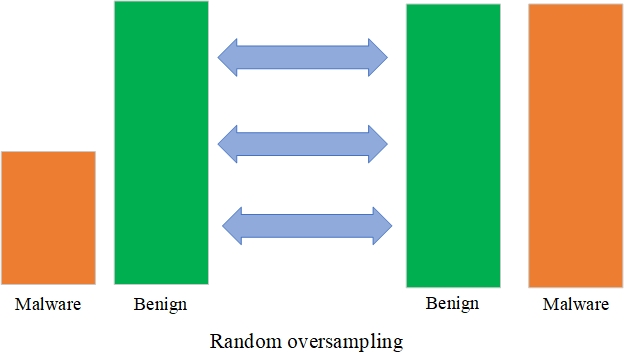
\includegraphics[width=0.6\textwidth]{media/ict/image38}
	\caption*{Figure 1-Class balancing with Random oversampling}
\end{figure}

\begin{multicols}{2}
{\bfseries Classification with machine learning and deep learning models.}
When the classes are balanced, the dataset is classified with machine
and deep learning models. There are several such models, among which the
most popular are Decision Tree, Random Forest, XgBoost, Dense neural
network (DNN), Gated recurrent unit (GRU) neural network, and Long
short-term memory (LSTM) neural network.

A Decision Tree {[}12{]} is a supervised machine-learning model for the
classification task. This model is structured like a tree, with internal
nodes representing decisions based on feature values, branches that
demonstrate the outcomes of those decisions, and leaf nodes of the final
prediction and output. The topmost node of the tree presents the entire
dataset, which is the starting point for decision-making and is split
based on the feature that provides the best separation of the data. At
the internal nodes, the dataset is split into two or more subgroups
based on the chosen feature's value. The final nodes do not further
split and correspond to a class label. The structure of the Decision
Tree is shown in Figure 2.
\end{multicols}

\begin{figure}[H]
	\centering
	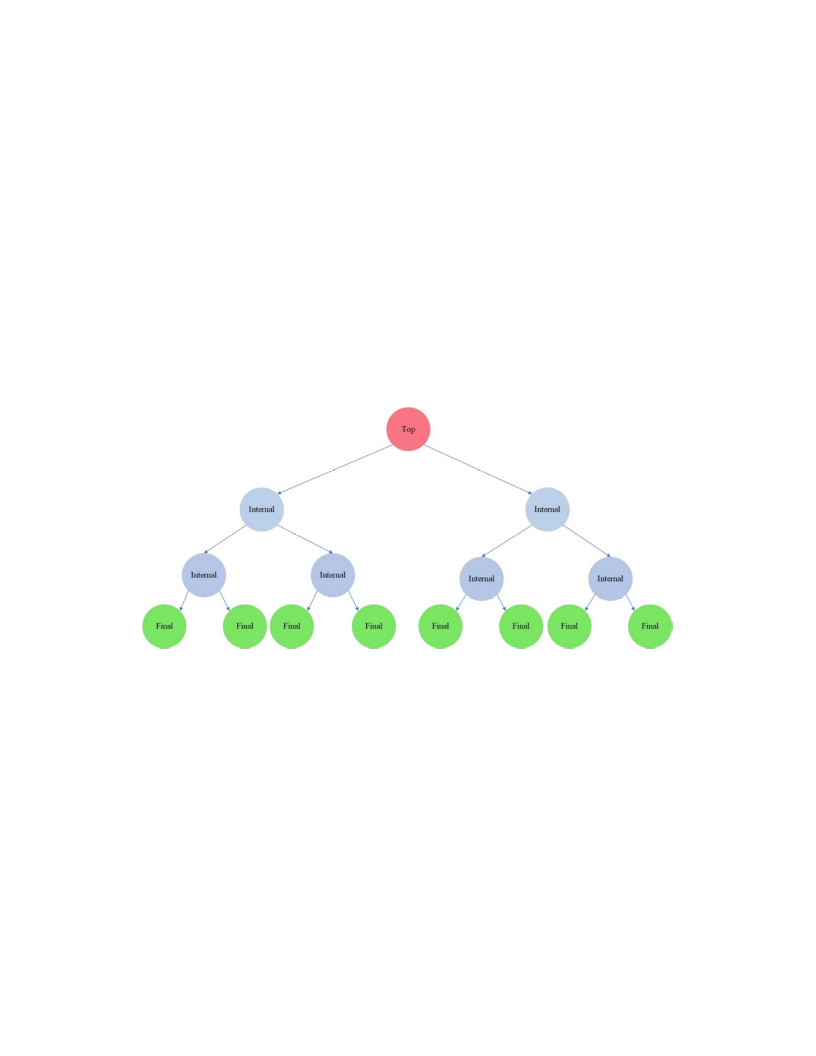
\includegraphics[width=0.85\textwidth]{media/ict/image39}
	\caption*{Figure 2-Decision Tree}
\end{figure}

\begin{multicols}{2}
A Random Forest {[}13{]} is a machine-learning algorithm that is based
on the concept of ensemble learning. It builds multiple decision trees
and combines their results to improve the Accuracy of a single decision
tree. The Random Forest algorithm uses bagging to create multiple
training datasets by randomly sampling from the original dataset with
replacement. Each decision tree is trained on a different bootstrapped
dataset, ensuring the trees are diverse and uncorrelated. Generally, the
Random Forest algorithm has the following specifications:

- It trains pretty quickly.

- It effectively processes datasets with a large number of features.

- It predicts data with very high Accuracy.

- It shows good efficiency even with a large number of missing data.

- It has high scalability.

The structure of Random Forest is shown in Figure 3.
\end{multicols}

\begin{figure}[H]
	\centering
	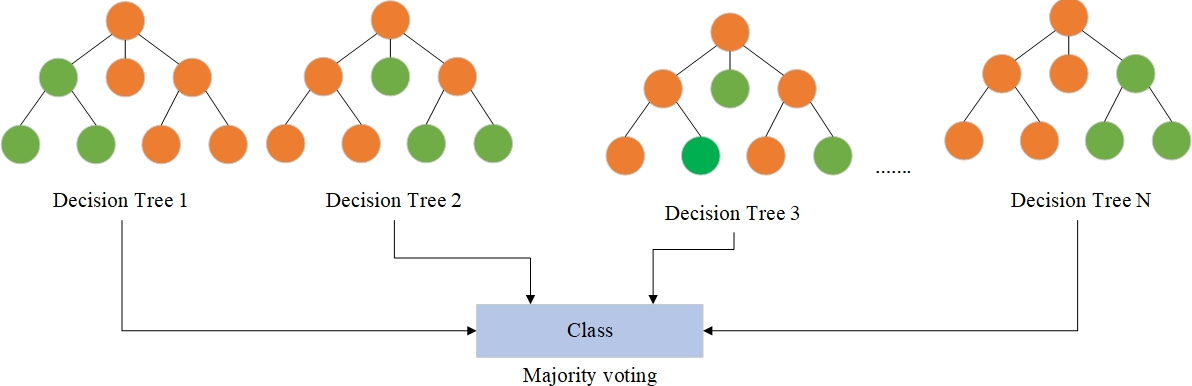
\includegraphics[width=0.9\textwidth]{media/ict/image40}
	\caption*{Figure 3 - Random Forest}
\end{figure}

\begin{figure}[H]
	\centering
	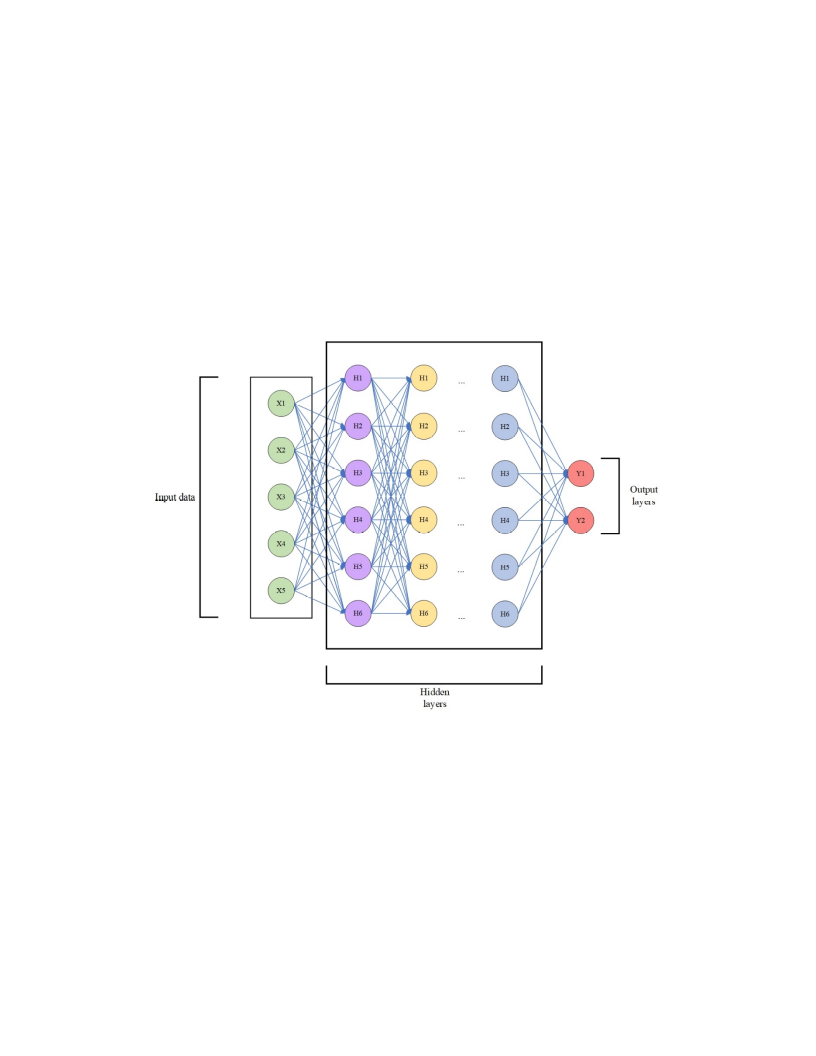
\includegraphics[width=0.75\textwidth]{media/ict/image44}
	\caption*{Figure 4 - Dense neural network}
\end{figure}

\begin{multicols}{2}
XGBoost {[}14{]} is a very strong machine-learning algorithm widely used
in the classification task. It lies in a series of boosting algorithms
that combine the predictions of multiple learners. XGBoost is known for
its efficiency and high performance. Employing an ensemble approach
corrects the errors made in previous iterations through the next model.
During each step, the deviations of the ensemble's predictions are
assessed on the training data, and the model is optimized by introducing
new tree forecasts to reduce the overall deviation. This process
continues until the desired error threshold is met or an early stopping
condition is triggered.

A Dense neural network (DNN) {[}15{]} is a fundamental type of neural
network in which each neuron in one layer is connected to every neuron
in the subsequent layer. It is the simplest architecture in neural
networks, typically used as the basic one in deep learning. In this
architecture, the input layer receives the input data $x=x_1,x_2,\ldots,x_n$, and $w_1,w_2,\ldots,w_n$ present weights of each level, and $b_1,b_2,\ldots,b_n$
of the input layer. The hidden layers consist of neurons that apply
weights to the input features, followed by an activation function that
produces non-linearity. There are usually many hidden layers in a neural
network. The output layer shows the final prediction that usually
corresponds to the number of classes: binary (two -- 0 or 1) and
multiclass (three or more). The scheme of DNN is presented in Figure 4.

A Long short-term memory (LSTM) {[}16{]} is a type of Recurrent neural
network designed to effectively capture long-term dependencies in the
sequential data and avoid problems related to the vanishing gradient. An
LSTM cell contains three types of gates: input, forget, and output,
which regulate the stream of information through the whole network. The
forget gate decides which information to discard from the cell state,
while the input gate selects new information to store. The output gate
defines the information that is required to be extracted from the
current cell state.
\end{multicols}

\begin{figure}[H]
	\centering
	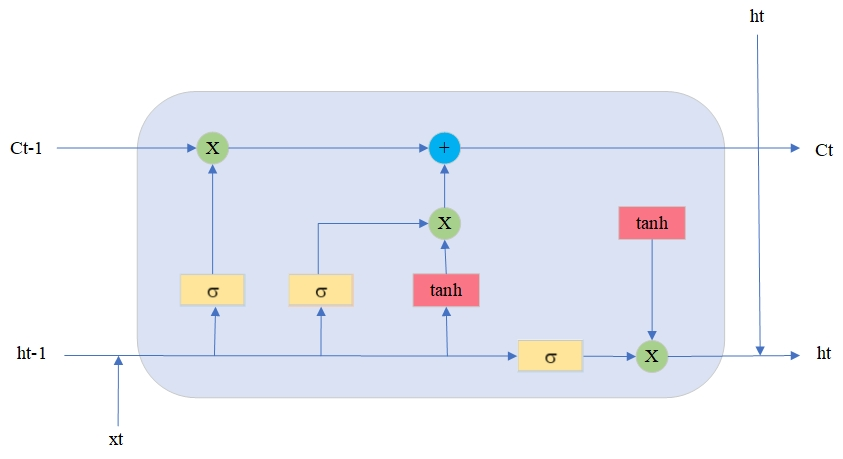
\includegraphics[width=0.6\textwidth]{media/ict/image63}
	\caption*{Figure 5 - Long short-term memory neural network}
\end{figure}

\begin{multicols}{2}
The forget gate is calculated as (4):

\begin{equation}
f_t=\sigma(W_f\cdot[h_{t-1},x_t]+b_f),
\end{equation}

where $f_t$ is a forget gate output;
$\sigma$ is a sigmoid activation function;
$W_f$ are weights for the forget gate;
$h_{t-1}$ state from the previous time step;
$x_t$ is a current input; $b_f$ is bias
for the forget gate.

The input gate is computed as (5):

\begin{equation}
i_t=\sigma(W_i\cdot[h_{t-1},x_t]+b_i),
\end{equation}

where $i_t$ is an input gate;
$W_i$ are weights for the input gate;
$b_i$ is bias for the input gate.

The cell state is calculated as (6):

\begin{equation}
C_t=tanh(W_c\cdot[h_{t-1},x_t]+b_c),
\end{equation}

where $C_t$ is a cell state;
$W_c$ are weights for the cell state;
$b_c$ is bias for the cell state.

The output gate is computed as (7):

\begin{equation}
o_t=\sigma(W_o\cdot[h_{t-1},x_t]+b_o),
\end{equation}

where $o_t$ is the output gate;
$b_o$ is bias for the output gate.

The scheme of the LSTM model is shown in Figure 5.

A GRU {[}17{]} is another type of Recurrent neural network designed to
capture dependencies in sequential data like LSTM but with a simpler
structure. GRU combines the hidden and cell states into one entity,
making them computationally more efficient than LSTM {[}18{]}. GRU
includes update, reset gates, candidate hidden state, and final hidden
state.

The update gate is calculated as (8):

\begin{equation}
z_t=\sigma(W_z\cdot[h_{t-1},x_t]+b_z),
\end{equation}

where $z_t$ is an update gate;
$\sigma$ is a sigmoid activation function;
$W_z$ is a weight matrix for the update gate.

The reset gate is computed as (9):

\begin{equation}
r_t=\sigma(W_r\cdot[h_{t-1},x_t]+b_r),
\end{equation}

where $r_t$ is a reset gate;
$W_r$ is a weight matrix for the reset gate;
$b_r$ is a bias for the reset gate.

The hidden state is calculated as (10):

\begin{equation}
\tilde{h_t}=tanh(W_h\cdot[r_t*h_{t-1},x_t]+b_h),
\end{equation}

where $\tilde{h_t}$ is a
candidate hidden state, which incorporates the current input and the
reset hidden state;
$W_h$ is the weight matrix for the candidate hidden state;
$b_h$ is a bias term for the candidate hidden state;
$*$ is the element-wise multiplication.

The final hidden state is computed as (11):

\begin{equation}
h_t=z_t*h_{t-1}+(1-z_t)*\tilde{h_t},
\end{equation}

where $h_t$ is a final hidden state for the current time step; $z_t$ is an update
gate controlling how much of the previous hidden state to keep and how
much of the candidate state to add.

The scheme of the GRU neural network is shown in Figure 6.
\end{multicols}

\begin{figure}[H]
	\centering
	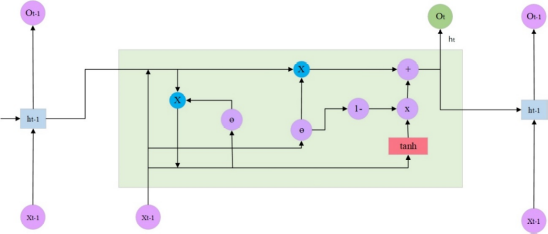
\includegraphics[width=0.6\textwidth]{media/ict/image79}
	\caption*{Figure 6 - Gated recurrent unit neural network}
\end{figure}

\begin{multicols}{2}
The machine learning and neural network algorithms presented above have
been widely used and distributed in many works due to their success in
data classification tasks. In this study, they also successfully coped
with the task of malware detection. However, to improve the efficiency
of threat detection, a new hybrid neural network model, which includes
LSTM and GRU layers, was developed. This model combines the advantages
of both architectures for more efficient data processing. The first
recurrent LSTM layer helps model long-term dependencies in data,
revealing patterns~useful for identifying threats. Since LSTM has
memory, it retains information about previous steps, which is especially
important in sequence analysis. The GRU layer follows LSTM and helps
simplify the model training by reducing the number of parameters
compared to LSTM, making it more efficient. The hybrid LSTM-GRU model
uses the advantages of both architectures. The LSTM layer is used as the
first layer to process the data, and the GRU can be used in the next
stage to speed up the training and processing of the output data. This
reduces the training time on large datasets. Overall, the hybrid
LSTM-GRU model offers enough functionality to handle complex models
without overloading the computational resources of the machines. The
scheme of the hybrid LSTM-GRU neural network model is shown in Fig. 7.
\end{multicols}

\begin{figure}[H]
	\centering
	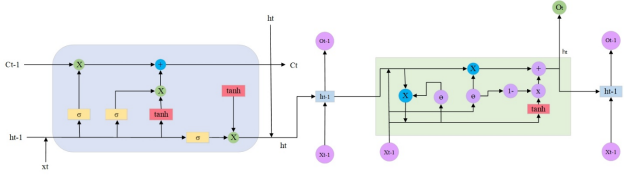
\includegraphics[width=0.8\textwidth]{media/ict/image80}
	\caption*{Figure 7 - LSTM-GRU neural network}
\end{figure}

\begin{multicols}{2}
{\bfseries Results and discussion.} Malware classification experiments
{[}19{]} were tested on the corresponding dataset. First of all, the
dataset was cleaned and preprocessed. Three unmeaning features were
eliminated, while the remaining 55 features were normalized with the
Min-Max scaling technique {[}20{]}. The feature selection algorithm was
applied to the normalized dataset, retrieving the 20 most significant
ones. In total, 3 machine learning (Decision Tree, Random Forest,
XgBoost), 3 deep learning (DNN, LSTM, and GRU), and 1 proposed hybrid
LSTM-GRU deep learning model were used to classify the dataset.

The results were evaluated with the use of 4 measures: Accuracy,
Precision, Recall, and F1-score. Accuracy measures the portion of
correctly classified elements out of the whole number of elements. The
formula for calculating Accuracy is shown in (12):

\begin{equation}
Accuracy=\frac{TP+TN}{Total \text{\_} number}
\end{equation}

Precision is the portion of correctly predicted positive elements to the
total elements that were predicted as positive. Precision is computed as
(13):

\begin{equation}
Precision=\frac{TP}{TP+FP}
\end{equation}

Recall is the portion of correctly predicted positive elements to the
total actual positive elements. Recall is computed as (14):

\begin{equation}
Recall=\frac{TP}{TP+FN}
\end{equation}

F1-score is the metric characterizing the balance between Precision and
Recall. F1-score is computed as (15):

\begin{equation}
F1- score =2\times\frac{Precision \times Recall}{Precision + Recall}
\end{equation}

The results of classifying the Malware dataset with machine learning and
deep learning models were evaluated with the described metrics, the
histograms, and the Area Under the ROC curve. The AUC-ROC value is in
the range of 0 to 1.0. A value of 1.0 means an ideal classifier; a value
of 0.5 describes random guessing, and a value less than 0.5 identifies a
problematic case.

The results of the experiments that were conducted are shown in Table 1
and Figure 7.
\end{multicols}

\begin{table}[H]
\caption*{Table 1. The values of Malware classification}
\centering
\begin{tabular}{|l|l|l|l|l|l|l|l|}
\hline
Metrics   & Decision Tree & Random Forest & XGBoost & DNN   & LSTM  & GRU   & \multirow{1}{2cm}{Proposed LSTM-GRU model} \\ \hline
Ассurасy  & 0.988         & 0.992         & 0.989   & 0.959 & 0.972 & 0.971 & 0.986                   \\ \hline
Рrесisiоn & 0.985         & 0.991         & 0.987   & 0.962 & 0.972 & 0.966 & 0.981                   \\ \hline
Rесаll    & 0.991         & 0.993         & 0.991   & 0.957 & 0.972 & 0.976 & 0.989                   \\ \hline
F1-sсоrе  & 0.988         & 0.992         & 0.989   & 0.960 & 0.972 & 0.971 & 0.985                   \\ \hline
\end{tabular}
\end{table}

\begin{figure}[H]
	\centering
	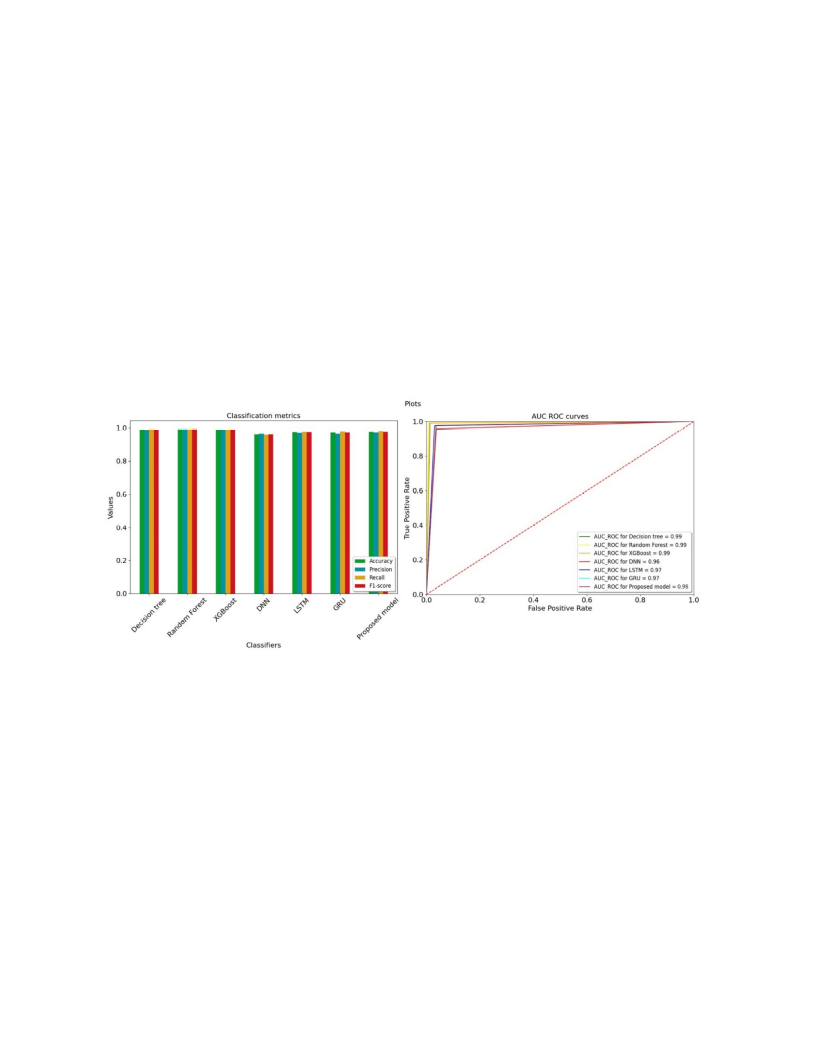
\includegraphics[width=0.8\textwidth]{media/ict/image85}
	\caption*{Figure 7-Histograms and an AUC-ROC curve}
\end{figure}

\begin{multicols}{2}
All seven models showed good classification results. The Decision Tree,
Random Forest, and XGBoost machine learning models gave high accuracy
scores. It proves that machine learning algorithms are still strong in
the classification tasks of the cybersecurity field. The Random Forest
model reached scores of 0.99, being the best among other machine
learning models. This proves that Random Forest has always had the
greatest potential in classification tasks. Among neural networks, the
simple DNN model was a little worse than LSTM and GRU by around 0.01.
The recurrent LSTM and GRU models showed mostly identical scores. The
proposed LSTM-GRU model outperformed other deep learning models by 0.01
and demonstrated good tendencies in getting even higher scores in case
of having larger datasets.

{\bfseries Conclusion.} The fast development of computer technologies has
led to the appearance of a large number of cyber threats that advance in
breaches of security and confidentiality of information systems. The
practical side of this research presents the creation and testing of
malware detection models that can improve the security and resilience of
information systems to modern cyber threats. Malware is one of the most
dangerous threats because many of its forms exist, including viruses,
worms, trojans, spyware, etc. They can rapidly spread in the information
environment. Therefore, effective measures of their detection and
prevention have become especially relevant in the last decade. The
traditional ways of protecting against such cyber threats have become
less significant in recent years. It is necessary to utilize other
advanced methods. This research is based on machine learning algorithms
and deep learning models, which allow the analysis of malware based on
known signatures and identify new, previously unknown threats. The
practical experiments of this research work covered the detection of
malware threats with the use of seven machine learning and deep learning
models, including Decision Tree, Random Forest, XGBoost, DNN, LSTM, GRU,
and the proposed hybrid LSTM-GRU, giving accuracy scores above 0.95. The
LSTM-GRU and Random Forest models reached scores of 0.98 and 0.99, being
very close to the ideal result. It is also planned to extend this
research, adding more experiments to classify various other types of
threats in future works. Therefore, the study demonstrates that using
machine learning and deep learning to analyze malware can improve the
accuracy and reliability of classification and increase the flexibility
of security systems, making them less vulnerable to new, unpredictable
threats.

\emph{{\bfseries Financing.} This work was carried out under project
AP19675957, titled ``The research and development of the system for
ensuring the protection of medical data using blockchain technology and
artificial intelligence methods,'' implemented at the Institute of
Information and Computational Technologies.}
\end{multicols}

\begin{center}
{\bfseries References}
\end{center}

\begin{references}
\begin{enumerate}
\def\labelenumi{\arabic{enumi}.}
\item
  Khando, K., Gao, S., Islam, S. M., \& Salman, A. Enhancing employees
  information security awareness in private and public organisations: A
  systematic literature review // Computers \& security. -2021.- Vol.
  106. DOI
  \href{https://doi.org/10.1016/j.cose.2021.102267}{10.1016/j.cose.2021.102267}.
\item
  Nissenbaum, H. Protecting privacy in an information age: The problem
  of privacy in public //In The ethics of information technologies.
  Routledge. -2020.- P. 141-178. DOI
  \href{https://doi.org/10.2307/3505189}{10.2307/3505189}.
\item
  Shelke, M.V., Deshmukh, J.Y., Ajalkar, D.A., \& Dhumal, R.B. A Robust
  Ensemble Learning Approach for Malware Detection and Classification //
  Journal of Advanced Research in Applied Sciences and Engineering
  Technology.-2024.-Vol. 48(1).- P. 152-167.
\end{enumerate}

DOI
\href{https://doi.org/10.37934/araset.48.1.152167}{10.37934/araset.48.1.152167}.

\begin{enumerate}
\def\labelenumi{\arabic{enumi}.}
\setcounter{enumi}{3}
\item
  Zhao, Q., Chen, S., Liu, Z., Baker, T., \& Zhang, Y. Blockchain-based
  privacy-preserving remote data integrity checking scheme for IoT
  information systems // Information Processing \& Management. -2020. -
  Vol. 57(6). \href{https://doi.org/10.1016/j.ipm.2020.102355}{DOI
  10.1016/j.ipm.2020.102355}.
\item
  Tun Li, Ya Luo, Xin Wan, Qian Li, Qilie Liu, Rong Wang, Chaolong Jia,
  Yunpeng Xiao. A malware detection model based on imbalanced
  heterogeneous graph embeddings // Expert Systems with
  Applications.-2024.-Vol. 246. 123109. DOI
  \href{https://doi.org/10.1016/j.eswa.2023.123109}{10.1016/j.eswa.2023.123109}.
\item
  Caixia Gao, Yao Du, Fan Ma, Qiuyan Lan, Jianying Chen, Jingjing Wu. A
  new adversarial malware detection method based on enhanced lightweight
  neural network // Computers \& Security. -2024. -Vol. 147. DOI
  \href{https://doi.org/10.1016/j.cose.2024.104078}{10.1016/j.cose.2024.104078}.
\item
  Wira Zanoramy, Mohd Faizal Abdollah, Othman Abdollah, \& S.M. Warusia
  Mohamed S.M.M. Ransomware Early Detection using Machine Learning
  Approach and Pre-Encryption Boundary Identification // Journal of
  Advanced Research in Applied Sciences and Engineering Technology.
  -2024. -Vol. 47(2).- P. 121 - 137. DOI
  \href{https://doi.org/10.37934/araset.47.2.121137}{10.37934/araset.47.2.121137}.
\item
  Hossain, M.A., Islam, M.S. Enhanced detection of obfuscated malware in
  memory dumps: a machine learning approach for advanced cybersecurity
  // Cybersecurity. -2024. -Vol. 7(16).
\end{enumerate}

DOI
\href{https://doi.org/10.1186/s42400-024-00205-z}{10.1186/s42400-024-00205-z}.

\begin{enumerate}
\def\labelenumi{\arabic{enumi}.}
\setcounter{enumi}{8}
\item
  Mosleh M. Abualhaj, Ahmad Sami Al-Shamayleh, Alhamza Munther, Sumaya
  Nabil Alkhatib, Mohammad O. Hiari, Mohammed Anbar\emph{.} Enhancing
  spyware detection by utilizing decision trees with hyperparameter
  optimization // Bulletin of Electrical Engineering and Informatics.
  -2022. -Vol. 13(5). - P. 3653-3662. DOI
  \href{https://doi.org/10.11591/eei.v13i5.7939}{10.11591/eei.v13i5.7939}.
\item
  Ahmad Heryanto, Deris Stiawan, Adi Hermansyah, Rici Firnando, Hanna
  Pertiwi, Mohd Yazid Bin Idris, Rahmat Budiarto The incorporation of
  stacked long short-term memory into intrusion detection systems for
  botnet attack classification // IAES International Journal of
  Artificial Intelligence. -2024. -Vol. 13(3).- P. 3657-3670. DOI
  \href{https://doi.org/10.11591/ijai.v13.i3.pp3657-3670}{10.11591/ijai.v13.i3.pp3657-3670}.
\item
  Aso Mafakheri, Sadegh Sulaimany. Android malware detection through
  centrality analysis of applications network//Applied Soft Computing.
  -2024.-Vol. 165.
\end{enumerate}

DOI
\href{https://doi.org/10.1016/j.asoc.2024.112058}{10.1016/j.asoc.2024.112058}.

\begin{enumerate}
\def\labelenumi{\arabic{enumi}.}
\setcounter{enumi}{11}
\item
  Singh, D., \& Singh, B. Investigating the impact of data normalization
  on classification performance // Applied Soft Computing. -2020. -Vol.
  97. DOI
  \href{https://doi.org/10.1016/j.asoc.2019.105524}{10.1016/j.asoc.2019.105524}.
\item
  Andelic, N., \& Baressi Šegota, S. Development of symbolic expressions
  ensemble for breast cancer type classification using genetic
  programming symbolic classifier and decision tree classifier //
  Cancers. -2023. - Vol. 15(13). DOI
  \href{https://doi.org/10.3390/cancers15133411}{10.3390/cancers15133411}.
\item
  Manzali, Y., \& Elfar, M. Random forest pruning techniques: a recent
  review // In Operations research forum. -2023. -Vol. 4(43). DOI
  \href{https://doi.org/10.1007/s43069-023-00223-6}{10.1007/s43069-023-00223-6}.
\item
  Hariharan, B., Siva, R., Sadagopan, S., Mishra, V., \& Raghav, Y.
  Malware Detection Using XGBoost based Machine Learning Models-Review
  // In 2023 2nd International Conference on Edge Computing and
  Applications (ICECAA). -2023. -P. 964-970.
\end{enumerate}

DOI
\href{https://doi.org/10.1109/ICECAA58104.2023.10212327}{10.1109/ICECAA58104.2023.10212327}.

\begin{enumerate}
\def\labelenumi{\arabic{enumi}.}
\setcounter{enumi}{15}
\item
  Gupta, K., Jiwani, N., Sharif, M. H. U., Datta, R., \& Afreen, N. A
  Neural Network Approach For Malware Classification // In 2022
  International Conference on Computing, Communication, and Intelligent
  Systems (ICCCIS). -2022. -P. 681-684.
\end{enumerate}

DOI
\href{https://doi.org/10.1109/ICCCIS56430.2022.10037653}{10.1109/ICCCIS56430.2022.10037653}.

\begin{enumerate}
\def\labelenumi{\arabic{enumi}.}
\setcounter{enumi}{16}
\item
  Catak, F. O., Ahmed, J., Sahinbas, K., \& Khand, Z. H. Data
  augmentation based malware detection using convolutional neural
  networks // Peerj computer science. - 2021.
\end{enumerate}

DOI \href{https://doi.org/10.7717/peerj-cs.346}{10.7717/peerj-cs.346}.

\begin{enumerate}
\def\labelenumi{\arabic{enumi}.}
\setcounter{enumi}{17}
\item
  Thakur, P., Kansal, V., \& Rishiwal, V. Hybrid deep learning approach
  based on lstm and cnn for malware detection // Wireless Personal
  Communications. -2024. -Vol. 136(3). - P.1879-1901. DOI
  \href{https://doi.org/10.1007/s11277-024-11366-y}{10.1007/s11277-024-11366-y}.
\item
  Kolli, S., Balakesavareddy, P., \& Saravanan, D. Neural Network based
  Obfuscated Malware detection // In 2021 International Conference on
  System, Computation, Automation and Networking (ICSCAN). -2021. DOI
  \href{https://doi.org/10.1109/ICSCAN53069.2021.9526496}{10.1109/ICSCAN53069.2021.9526496}.
\item
  Ussatova, O., Zhumabekova, A., Begimbayeva, Y., Matson, E. T., \&
  Ussatov, N. Comprehensive DDoS Attack Classification Using Machine
  Learning Algorithms // Computers, Materials \& Continua. -2022. -Vol.
  73(1). - P. 577-594. DOI
  \href{https://doi.org/10.32604/cmc.2022.026552}{10.32604/cmc.2022.026552}.
\item
  Ussatova, O., Zhumabekova, A., Karyukin, V., Matson, E. T., Ussatov,
  N. The development of a model for the threat detection system with the
  use of machine learning and neural network methods //International
  Journal of Innovative Research and Scientific Studies. -2024.-Vol.
  7(3). -P. 863- 877. DOI
  \\\href{https://doi.org/10.53894/ijirss.v7i3.2957}{10.53894/ijirss.v7i3.2957}.
\end{enumerate}
\end{references}

\begin{authorinfo}
\hspace{1em}\emph{{\bfseries Information about the authors}}

Zhumabekova A.- мaster, Institute of Information and Computational
Technologies, Al-Farabi Kazakh National University, Almaty, Kazakhstan,
e-mail:
\href{mailto:zhumabekova2702@gmail.com}{\nolinkurl{zhumabekova2702@gmail.com}};

Ussatova O.- PhD, associate professor, Institute of Information and
Computational Technologies, G.Daukeev Almaty University of Energy and
Communications, Almaty, Kazakhstan\emph{,} e-mail:
\href{mailto:uoa_olga@mail.ru}{\nolinkurl{uoa\_olga@mail.ru}};

Kalimoldayev M. -- doctor of Physical and Mathematical Sciences,
professor, Academician of the National Academy of Sciences of the
Republic of Kazakhstan, Institute of Information and Computational
Technologies, Almaty, Kazakhstan, e-mail:
\href{mailto:mnk@ipic.kz}{\nolinkurl{mnk@ipic.kz}};

Karyukin V.-PhD, Institute of Information and Computational
Technologies, Al-Farabi Kazakh National University, Almaty, Kazakhstan,
e-mail:
\href{mailto:vladislav.karyukin@gmail.com}{\nolinkurl{vladislav.karyukin@gmail.com}};

Begimbayeva Y.-PhD, Associate professor, Institute of Information and
Computational Technologies, G.Daukeev Almaty University of Energy and
Communications, Almaty, Kazakhstan\emph{,} Almaty, Kazakhstan, e-mail:
\href{mailto:Enlik_89@mail.ru}{\nolinkurl{Enlik\_89@mail.ru}}

\hspace{1em}\emph{{\bfseries Сведения об авторах}}

Жұмабекова А.Т.-магистр, Институт информационных и вычислительных
технологий, КазНУ им. аль-Фараби, Алматы, Казахстан, e-mail:
\href{mailto:zhumabekova2702@gmail.com}{\nolinkurl{zhumabekova2702@gmail.com}};

Усатова О.А. - PhD, ассоциированный профессор (доцент), Институт
информационных и вычислительных технологий, Алматинский Университет
Энергетики и Связи им. Г.Даукеева,Алматы, Казахстан, e-mail:
\href{mailto:uoa_olga@mail.ru}{\nolinkurl{uoa\_olga@mail.ru}};

Калимолдаев М.Н.- доктор физико-математических наук, профессор, Академик
НАН РК, Институт информационных и вычислительных технологий, Алматы,
Казахстан, e-mail: \href{mailto:mnk@ipic.kz}{\nolinkurl{mnk@ipic.kz}};

Карюкин В.И.- PhD, Институт информационных и вычислительных технологий,
КазНУ им. аль-Фараби, Алматы, Казахстан, e-mail:
\href{mailto:vladislav.karyukin@gmail.com}{\nolinkurl{vladislav.karyukin@gmail.com}};

Бегимбаева Е.Е. - PhD, ассоциированный профессор (доцент), Институт
информационных и вычислительных технологий, Алматинский Университет
Энергетики и Связи им. Г.Даукеева, Алматы, Казахстан, e- mail:
\href{mailto:Enlik_89@mail.ru}{\nolinkurl{Enlik\_89@mail.ru}}
\end{authorinfo}
